\subsubsection{Progress}

During the previous weeks I have continued to work on on building a system model to simulate data transmission using conventional transmission techniques utilising the same optical channel model used for our autoencoder simulations. The purpose of this model is to provide a comparison between the performance of our autoencoders compared to conventional systems used in the industry.

\begin{itemize}
    \item \textbf{4PAM System Simulation}
    
    I have implemented demodulation techniques to my existing model, firstly by applying a 5th order Bessel filter with cutoff frequency 1/10 of the symbol rate to eliminate high frequency noise due to the optical channel. Pulse shaping is applied before decisions are made for each symbol based on decision levels placed midway between each possible signal level.
    
    \begin{figure}[H]
	\centering
	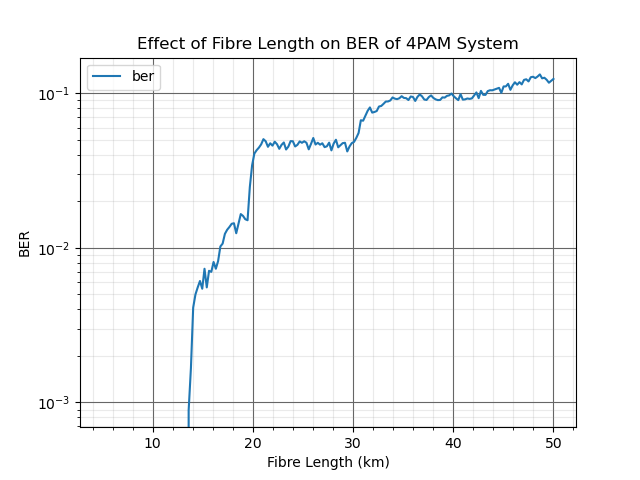
\includegraphics[width=0.9\textwidth]{Fibre Length vs BER.png}
	\caption{Plot of Bit Error Rate of 4PAM system against the fibre length of optical channel}
	\label{fig:output_signal}	
    \end{figure}
    
    By varying the length of the optical channel, the relationship between fibre length and BER can be seen from Figure \ref{fig:output_signal} which will prove to be useful in comparing the performance of the autoencoder system to 4PAM at different cable lengths. The simulation also allows the effects of varying noise and amount of dispersion experienced in the channel to be investigated.
    
    \item \textbf{2PAM System Simulation}
    
    I then changed the system for the 4PAM modulation scheme and reduced it down to provide a 2PAM system that also utilises the same optical channel model used for the autoencoder. 
    
    \item \textbf{OFDM System Simulation}
    
    \begin{figure}[H]
	\centering
	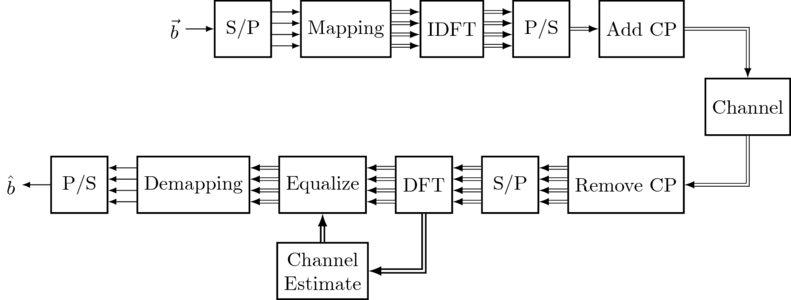
\includegraphics[width=0.9\textwidth]{OFDM diagram.png}
	\caption{Block Diagram containing fundamental blocks for OFDM system}
	\label{fig:OFDM}	
    \end{figure}
    
    The task I am currently working on has been in applying Orthogonal frequency-division multiplexing (OFDM) into a similar system simulation as 2PAM/4PAM which has proved to be more challenging. Time was taken in reading papers and online lectures to understand the concept of OFDM before attempting to apply it in python. I have been implementing each stage of Fig \ref{fig:OFDM} accordingly.
    
    The system utilises 16 QAM modulation scheme and transmits data over 64 subcarriers. Cyclic Prefix is also applied between adjacent OFDM symbols in order to inhibit inter-symbol interference with 25\% of each symbol being the cyclic prefix. Currently I have tested my system on a simple wireless channel that includes an impulse response channel convoluted onto the transmit signal with some additive noise. The next step is to implement the optical channel used in the autoencoder rather than the wireless network and similarly to the 2PAM/4PAM, investigate how the fibre length affects the BER of the system.
\end{itemize}